\section{Le projet déjà existant}
\paragraph{} \hspace{10mm}
A mon arrivée en Septembre, le projet avait déjà été amorcé par deux étudiants, \textbf{Gabriel Garcia} et \textbf{Guillaume Ruff}. Le premier à avoir travaillé sur le projet est Gabriel lors de son stage ST40, et est à l'origine de la base de donnée déjà existante ainsi que d'une interface web réalisée avec le framework Vue.js. Guillaume quant à lui, a recréé le site web dans le cadre d'une UV HEDT avec le framework Angular, afin d'avoir un site plus robuste et facile à maintenir.
La première phase du stage a donc consisté à finaliser ces deux projets en vue d'avoir une application web fonctionnelle et avec des interfaces abouties.

\subsection{Le backend : Django}

\setcounter{secnumdepth}{3}
\subsubsection{Présentation et avancement au début du stage}
\paragraph{} \hspace{10mm}
Lors de son stage, Gabriel a travaillé sur le développement d'un modèle relationnel sur le framework Django. Le modèle est divisé en deux sous-modèles : \textbf{Community} et \textbf{Database}. Le premier permet de gérer les utilisateurs, leurs droits et leurs identifiants et le deuxième permet de gérer tout ce qui est lié aux données. 

Le sous-modèle "Community" était déjà fonctionnel et achevé au début du stage : il permet d'avoir toutes les informations nécessaires sur les utilisateurs.

\begin{figure} [H]
    \centering
    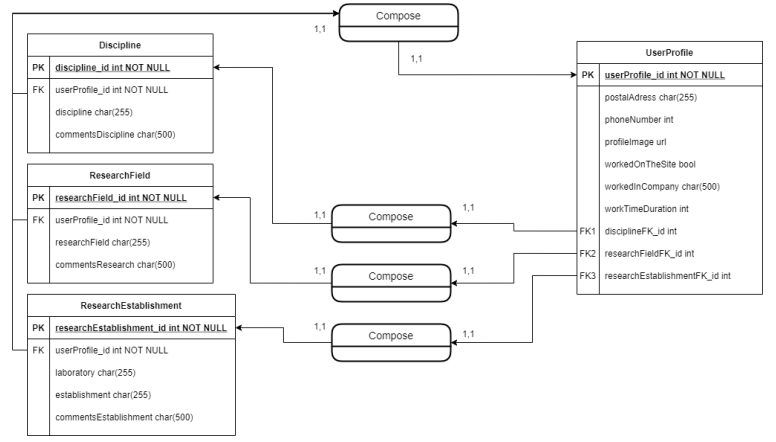
\includegraphics[width=1\textwidth]{assets/web/diagramme_modele_community.png}
    \caption{Diagramme de classe du sous-modèle relationnel "Community"}
    \caption*{\textbf{Source :} Gabriel Garcia}
    \label{fig:diagrammeClasseCommunity}
\end{figure}

\paragraph{} \hspace{10mm}
En revanche, en ce qui concerne la partie \textbf{Database}, tout n'était pas fonctionnel et terminé. Tout d'abord, nous avons très vite remarqué des problèmes de normalisations, qu'elles soient relationnelles ou syntaxiques. En témoigne la capture d'écran suivante, il y avait par exemple la table \textbf{Date} qui avait certains de ses champs dupliqués :

\begin{figure} [H]
    \centering
    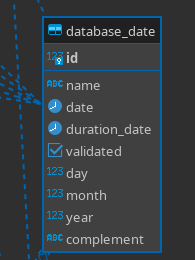
\includegraphics[width=0.175\textwidth]{assets/web/table_date.png}
    \caption{Capture d'écran de la table date du diagramme de classe du sous-modèle "Database"}
    \label{fig:tableDateDatabase}
\end{figure}

Comme on peut le voir, la table se compose d'un champ "date" de type Date ainsi que de trois champs "day", "month" et "year" de type Nombre. Les trois champs de type Nombre sont complètement inutiles et par conséquent la base de données ne respecte pas la forme normale 1FN.

Outre l'absence de forme normale du modèle, le code n'était lui non plus pas normalisé : certains champs des tables étaient déclarés en \textbf{Lower camel case}, et d'autres en \textbf{Upper camel case} ou en \textbf{Snake case}.

Enfin, les tests écrits par Gabriel relevaient 27 erreurs dont 22 liées à la table "source" ou à la table "source type".

\paragraph{} \hspace{10mm}
Dans l'ensemble l'essentiel du travail avait déjà été réalisé, comme on peut le voir ci-après même si tout n'est pas parfait. Dans un premier temps, notre tâche a été de tout normaliser et de "lisser" le code afin de le rendre plus clair. Ensuite, l'absence d'historien pour aider Gabriel s'est aussi faite sentir lorsque Cyril Lachèze est arrivé : dès les premières réunions nous avons vu que l'état dans lequel était le modèle ne permettrait pas d'enregistrer des données avec une granularité (i.e. le niveau de précision) convenable. Il fallait donc que l'on trouve une solution pour cela.

\begin{figure} [H]
    \centering
    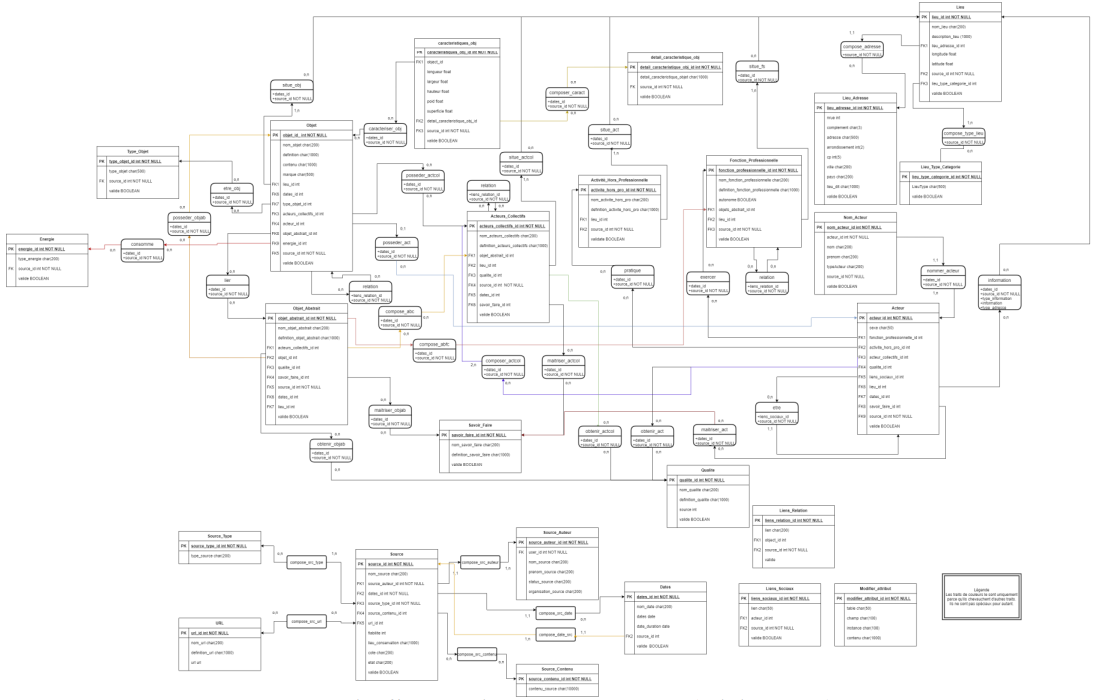
\includegraphics[width=1\textwidth]{assets/web/diagramme_modele_database.png}
    \caption{Diagramme de classe du sous-modèle relationnel "Database"}
    \caption*{\textbf{Source :} Gabriel Garcia}
    \label{fig:diagrammeClasseDatabase}
\end{figure}

\subsubsection{Le travail à effectuer}
\paragraph{} \hspace{10mm}
Pour rendre la base de données fonctionnelle, nous avons effectué plusieurs tâches clés. Tout d'abord, nous avons corrigé les bugs affectant les tables "source" et "source type". Ces bugs nous ont posés beaucoup de difficultés, qui peuvent être expliquées par trois facteurs :
\begin{itemize}
    \item[\ding{103}] premièrement, les migrations effectuées tout au long du développement du modèle étaient "corrompues". Au fil des modifications de ces deux tables, des coquilles se sont insérées dans le code des migrations ce qui les empêchaient de bien s'appliquer, résultant de l'apparition d'erreurs.
    \item[\ding{103}] deuxièmement, le champ liant la table "source type" à la table source était mal déclaré, ce qui a décuplé notre incompréhension vis-à-vis des erreurs si l'on prend en compte le premier point.
    \item[\ding{103}] enfin, ma non-maîtrise de django au début du stage et mon manque d'expérience en tant que développeur m'ont fait perdre beaucoup de temps. Connaissant mal le framework, j'ai par exemple mis plusieurs jours avant de comprendre l'intérêt du fichier \textbf{admin.py} et celui de dé-commenter la ligne qui ajoutait la table "source" au panneau d'administrateur, ce qui m'a par la suite beaucoup aidé à débugger les erreurs.  
\end{itemize}
\paragraph{} \hspace{10mm}
Ensuite, nous avons dû revoir les noms des champs avec Cyril. Ceux-ci n'étaient pas toujours explicites (voire pas du tout) et leur utilité n'était pas systématiquement expliqué dans le rapport de stage de Gabriel, il fallait donc les modifier (la figure 3.2 est un bon exemple : à ce jour, je n'ai toujours pas très bien compris l'intérêt du champ "duration\_date"). Cyril avait commencé à travailler sur ce sujet mais mon séjour à Nantes l'a interrompu suite à l'abandon de la base.
\paragraph{} \hspace{10mm}
En parallèle, nous avons également corrigé les erreurs dans les tests unitaires qui nous ont menés à une compréhension erronée du fonctionnement. Certains fonctionnent de nouveau mais il y a encore 5 tests défaillants : ils retournent une erreur alors qu'en pratique tout fonctionne. Nous n'avons pas réussi à les corriger, par conséquent nous les avons laissé tels quels et nous avons ajouté un commentaire dans le code indiquant qu'il fallait ignorer l'erreur.

\subsection{Le frontend : Angular (et Vue.Js)}

\subsubsection{Présentation et avancement au début du stage}
\paragraph{} \hspace{10mm}
Lorsque mon stage a débuté en septembre, deux interfaces avaient été conçues sous la forme de sites web. La première, implémentée par Gabriel, utilisait le framework \textbf{Vue.Js} et n'était pas totalement achevée : la structure globale du site était fonctionnelle mais les formulaires n'étaient pas exactement terminés et de nombreux petits détails pouvaient être corrigés afin d'améliorer l'expérience utilisateur.

\begin{figure} [H]
    \centering
    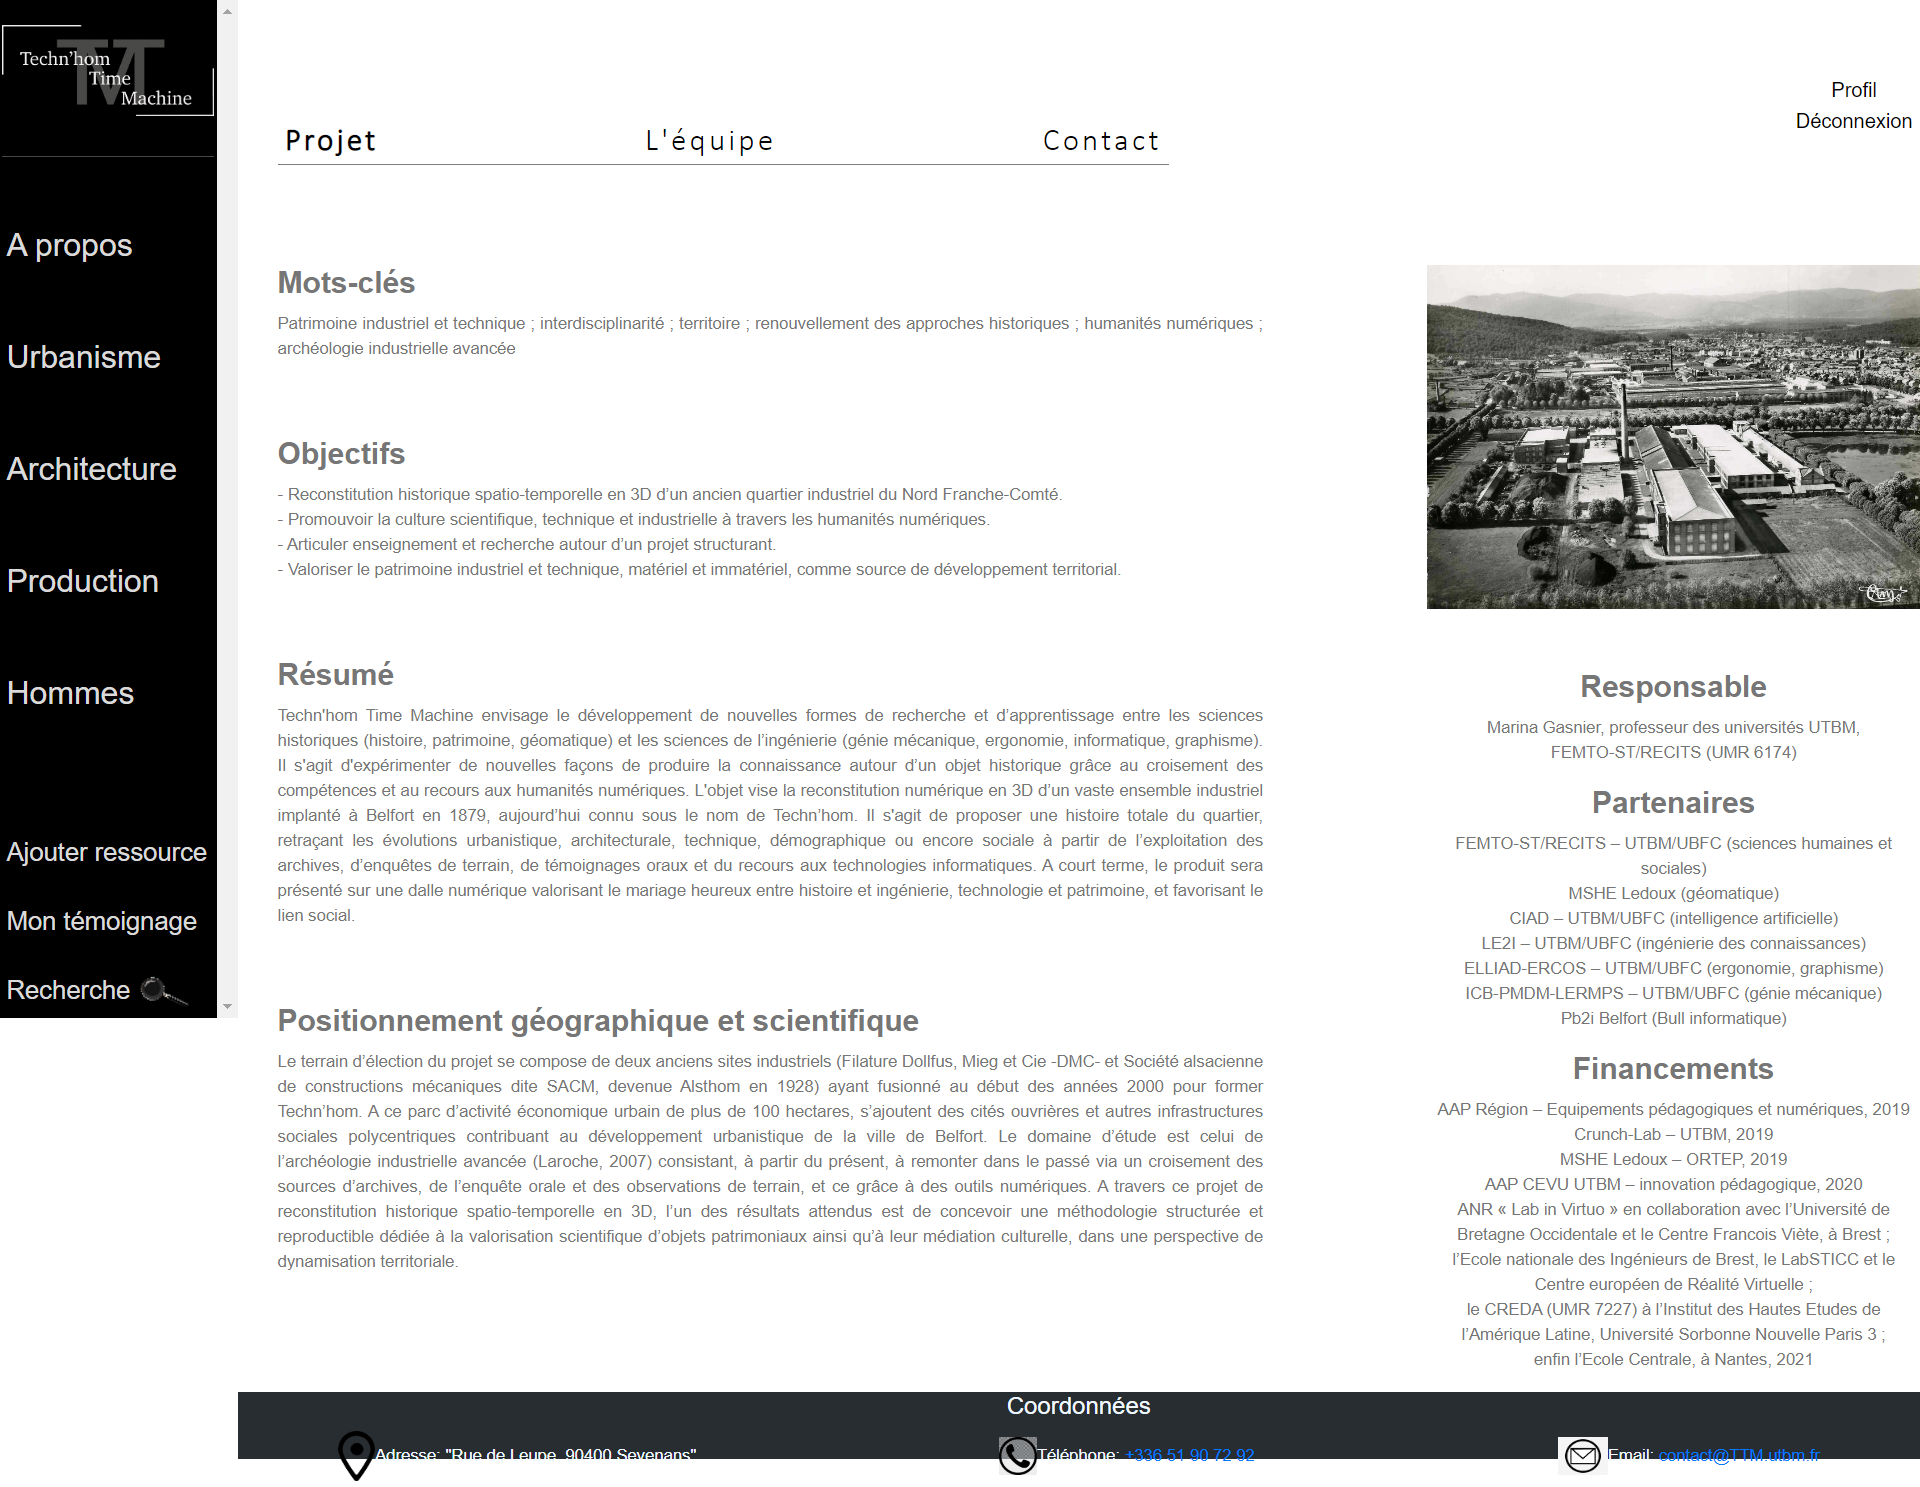
\includegraphics[width=1\textwidth]{assets/web/screen_main_vue.png}
    \caption{Capture d'écran de la page "A Propos" du site réalisé en Vue.Js}
    % \caption*{\textbf{Source :} Gabriel Garcia}
    \label{fig:screenMainVue}
\end{figure}

\Note{Le screenshot étant effectué avec une extension chrome qui "déroule" la page pour tout voir, on ne peut en fait pas tout lire sans défiler et le bandeau de gauche n'est pas trop petit}

\paragraph{} \hspace{10mm}
Nous pouvons voir sur cet exemple que plusieurs aspects peuvent être améliorés, comme les boutons \textbf{Profil} et \textbf{Déconnexion} qui ne sont pas très esthétiques ni très bien disposés. Le pied de page pourrait également être mieux façonné, tant sur la qualité des icônes que sur l'alignement du texte.

\paragraph{} \hspace{10mm}
Suite au stage de Gabriel, c'est ensuite Guillaume qui a poursuivi le projet au travers de l'UV HN2B. Son objectif tout au long du semestre avait été de recréer le site avec le framework \textbf{Angular}, Vue.Js ayant été jugé moins stable et moins maintenable. Ici aussi, Guillaume n'a pas pu achever son travail : aucune interface permettant d'afficher les données ni aucun formulaire n'avait été réalisé, il fallait donc tout designer et implémenter pour que l'ensemble soit opérationnel.

Voici à titre de comparaison la page "A propos" du site de Guillaume : 
\begin{figure} [H]
    \centering
    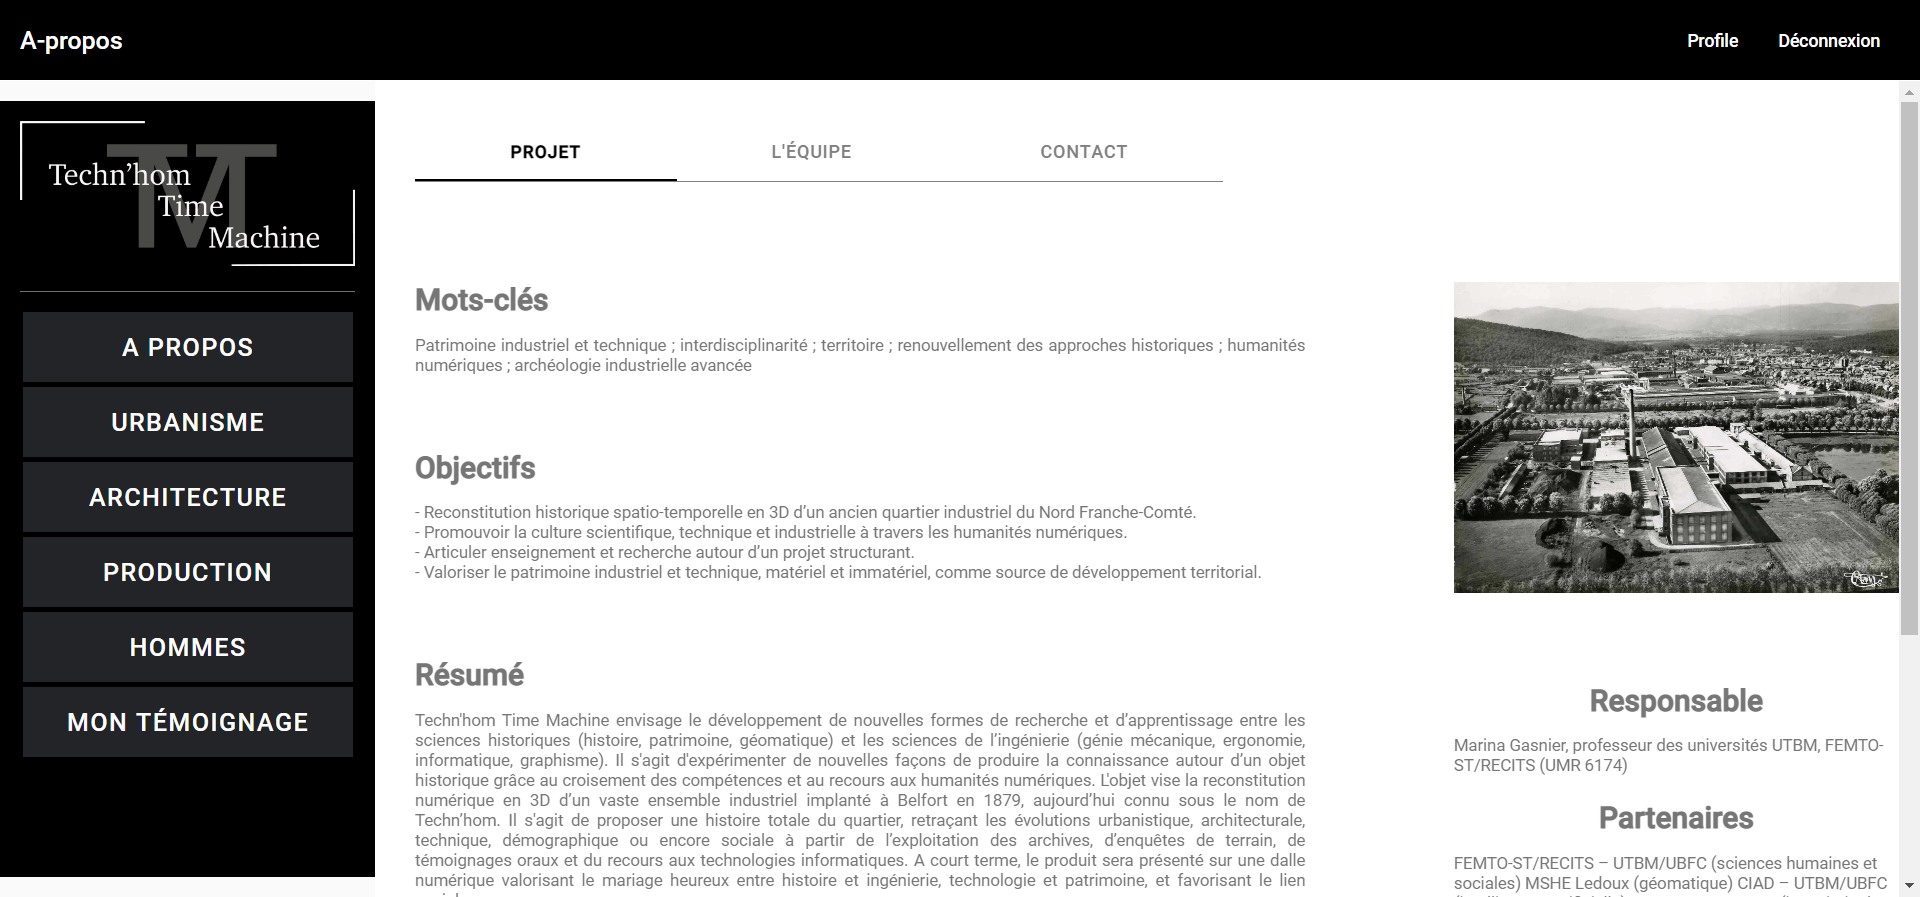
\includegraphics[width=1\textwidth]{assets/web/screen_main_angular.png}
    \caption{Capture d'écran de la page "A Propos" du site réalisé en Angular}
    % \caption*{\textbf{Source :} Gabriel Garcia}
    \label{fig:screenMainAngular}
\end{figure}

\subsubsection{Le travail à effectuer}
\paragraph{} \hspace{10mm}
Afin de finir le site, nous avons dû terminer deux tâches importantes : designer et implémenter les formulaires de saisies de données ainsi que les interfaces pour afficher ces mêmes données. Contrairement à Gabriel, nous n'avons pas souhaité utiliser Figma au vu de ce qu'il a pu en dire dans son rapport : ne sachant pas utiliser le logiciel et Figma ne permettant pas d'extraire du code HTML de bonne qualité, nous avons préféré designer nous-même interfaces et formulaires en se basant sur ce qui avait déjà été fait, c'est-à-dire, reproduire (dans un premier temps au moins) les formulaires de Gabriel tels quels tout en appliquant le nouveau style UI de Guillaume.

Pour plus d'efficacité, nous avons pensé que tout implémenter pour une des trois sections (Architecture, Production, Hommes) avant de passer à la section d'après était une meilleure idée que de créer tous les formulaires puis toutes les interfaces d'affichage, car cela nous éviterait d'avoir à effectuer trois fois les mêmes modifications en cas d'imprévu dans le design de ceux-ci. 

\paragraph{} \hspace{10mm}
La première (et unique) section que nous avons commencé à traiter est la section "Hommes". Dans un premier temps, nous avons pensé l'interface générale d'affichage des données puis l'interface d'affichage des détails. Seule la page affichant la liste des acteurs est terminée, mon séjour à Nantes ayant interrompu le développement du site, comme on peut le voir sur les figures 3.6 et 3.7 ci-après.

Par ailleurs, pour les mêmes raisons, aucun formulaire n'a pu être ébauché.
\begin{figure} [H]
    \centering
    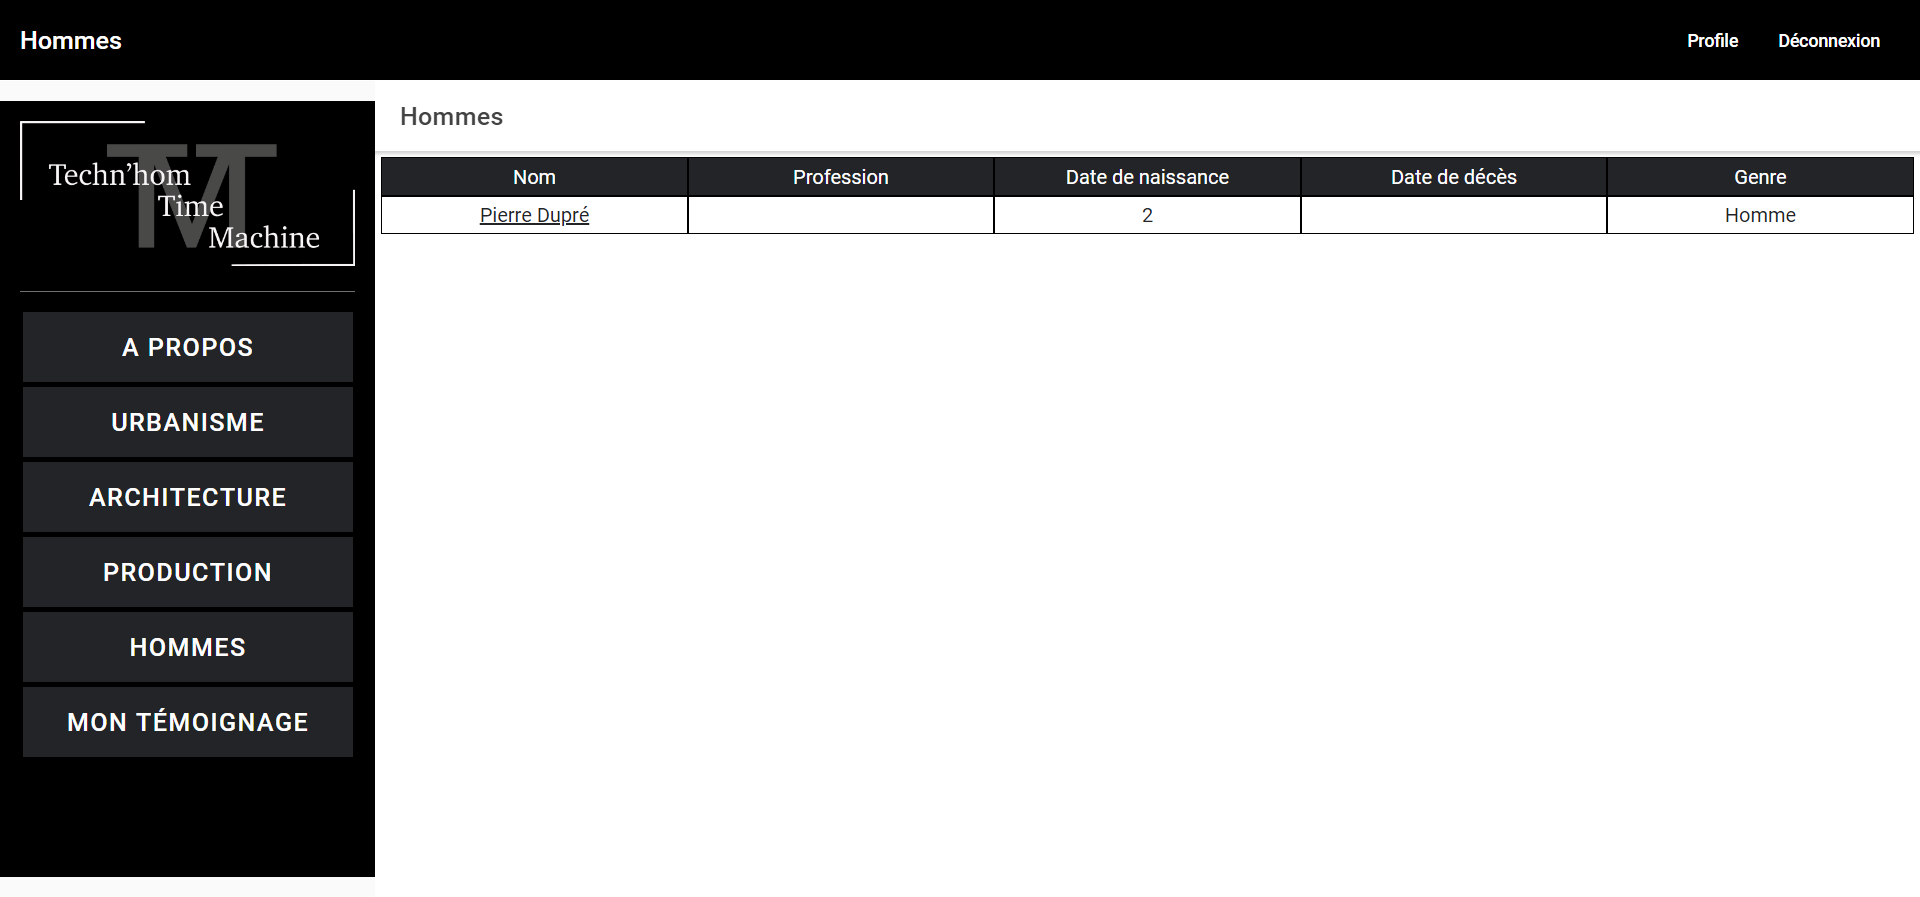
\includegraphics[width=1\textwidth]{assets/web/site/screen_liste_hommes.png}
    \caption{Capture d'écran de la page "Hommes" du site affichant les Acteurs}
    \label{fig:screenPageHommes}
\end{figure}

\begin{figure} [H]
    \centering
    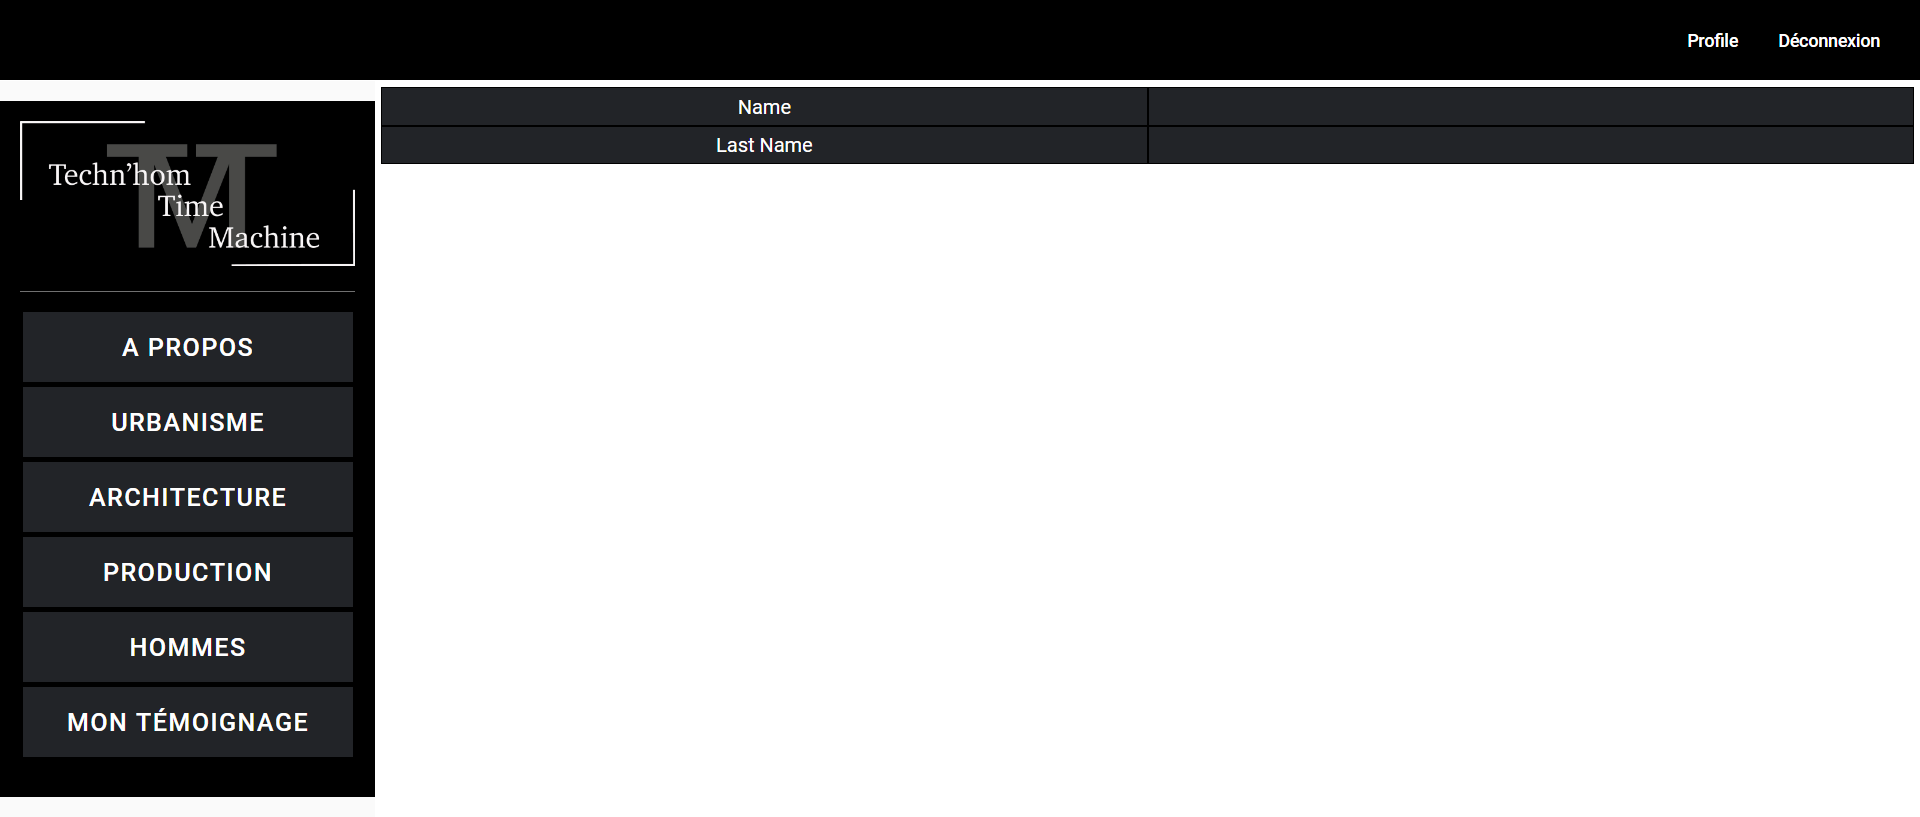
\includegraphics[width=1\textwidth]{assets/web/site/screen_detail_hommes.png}
    \caption{Capture d'écran de la page de détail d'un des acteurs de la page "Hommes"}
    \label{fig:screenPageHommesDetails}
\end{figure}

\pagebreak
\subsection{Problématique rencontrée}

\paragraph{} \hspace{10mm}
Pendant la semaine du 7 novembre, nous avons pris conscience que certains éléments ne convenaient pas dans le projet dans son état actuel. 

Tout d'abord, le modèle de la base de données n'était pas aussi abouti que nous le pensions. L'inconvénient d'un modèle relationnel (comparé à un modèle ontologique que nous aborderons après), est qu'il est beaucoup trop rigide pour le projet. Par conséquent, pour enregistrer par exemple deux objets qui ont des caractéristiques communes et des caractéristiques qui leur sont propres, nous avons deux solutions : soit créer une table commune aux deux avec tous les champs nécessaires, soit créer deux tables distinctes. Le problème de la première est son manque de "propreté" : ce n'est pas pratique d'utiliser une telle méthode car cela créerait des formulaires à rallonge dont la plupart des champs ne serviraient pas à chaque fois. Quant à la seconde, elle est mauvaise également car cela impliquerait de créer un nombre colossal de tables, ce qui n'est pas viable. Au final, aucune solution de convient pour un problème aussi basique.

Ensuite, les formulaires posaient aussi problème. Après avoir analysé le code de Gabriel, nous avons remarqué qu'il nous était impossible par exemple de lier plusieurs objets d'une certaine table à un objet d'une autre table à cause de la séparation du site en trois parties (Hommes, Architecture, Production).

Enfin, contrairement à ce qui était prévu dans le sujet de stage, il n'existe aucun outil d'échange entre une base relationnelle et Omeka-S. Par conséquent, il aurait fallu en créer un ce qui aurait pris beaucoup trop de temps et ne m'aurait pas permis d'atteindre mes objectifs de fin de stage. La seule autre option pertinente aurait été un triple-store, mais cela ne correspondait pas non plus au sujet initial.

Fort heureusement, mon séjour à Nantes a provoqué un tournant et nous avons pu repartir sur de nouvelles bases pour le projet grâce à Matthieu Quantin et l'utilisation des vocabulaires ouverts liés, aussi appelés ontologies.
